%!TeX root=../acctop.tex
%!TeX root=../acctop.tex
\addchap[Stave III: The Second of the Three Spirits]{{\moderatelyhuge Stave Three}\\ The Second of the Three Spirits}
\begin{minipage}[c]{\textwidth}
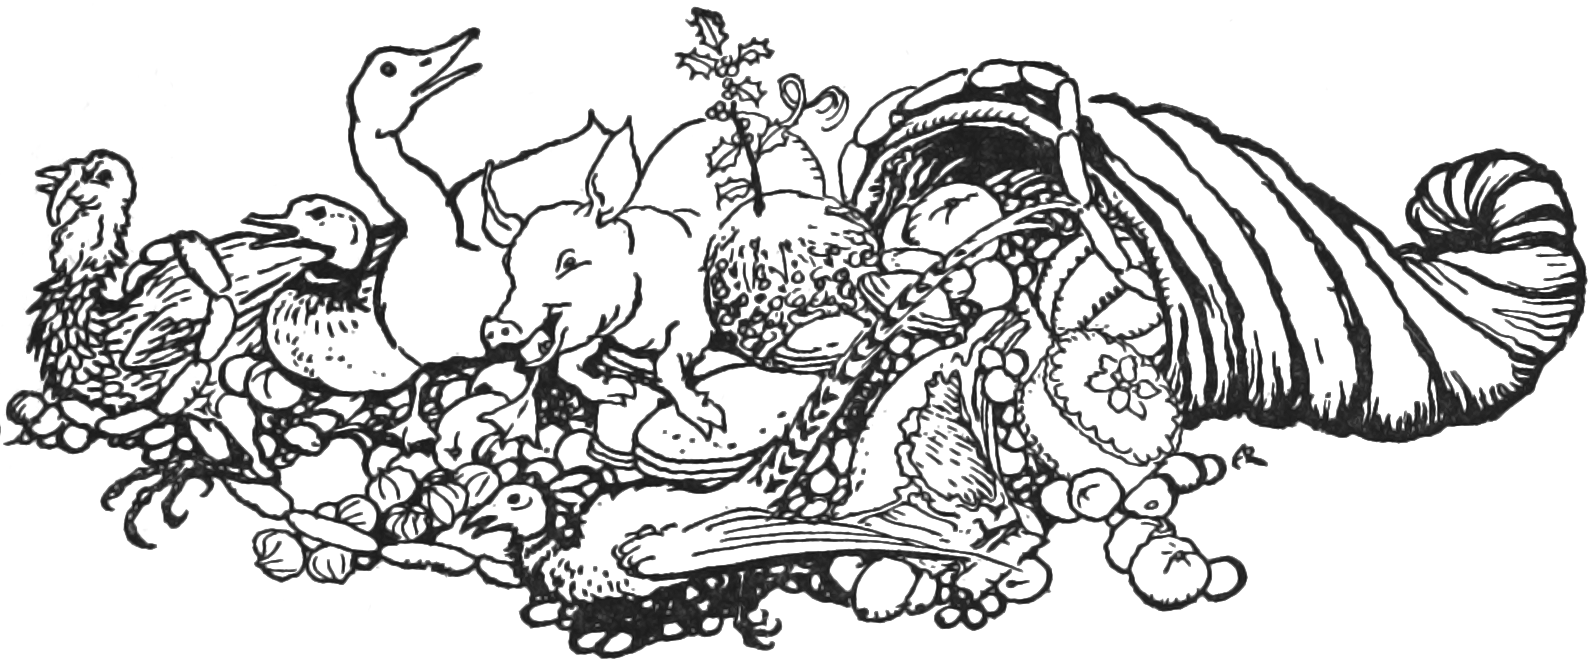
\includegraphics[width=\textwidth]{cornucopia}
\captionof{figure}[Headpiece to Stave III]{}
\end{minipage}
\vfill

\lettrine[lines=4]{A}{waking} in the middle of a prodigiously tough snore, and sitting up in bed to get his thoughts together, Scrooge had no occasion to be told that the bell was again upon the stroke of One. He felt that he was restored to consciousness in the right nick of time, for the especial purpose of holding a conference with the second messenger despatched to him through Jacob Marley's intervention. But finding that he turned uncomfortably cold when he began to wonder which of his curtains this new spectre would draw back, he put them every one aside with his own hands, and, lying down again, established a sharp look-out all round the bed. For he wished to challenge the Spirit on the moment of its appearance, and did not wish to be taken by surprise and made nervous.

Gentlemen of the free-and-easy sort, who plume themselves on being acquainted with a move or two, and being usually equal to the time of day, express the wide range of their capacity for adventure by observing that they are good for anything from pitch-and-toss to manslaughter; between which opposite extremes, no doubt, there lies a tolerably wide and comprehensive range of subjects. Without venturing for Scrooge quite as hardily as this, I don't mind calling on you to believe that he was ready for a good broad field of strange appearances, and that nothing between a baby and a rhinoceros would have astonished him very much.

Now, being prepared for almost anything, he was not by any means prepared for nothing; and consequently, when the bell  struck One, and no shape appeared, he was taken with a violent fit of trembling. Five minutes, ten minutes, a quarter of an hour went by, yet nothing came. All this time he lay upon his bed, the very core and centre of a blaze of ruddy light, which streamed upon it when the clock proclaimed the hour; and which, being only light, was more alarming than a dozen ghosts, as he was powerless to make out what it meant, or would be at; and was sometimes apprehensive that he might be at that very moment an interesting case of spontaneous combustion, without having the consolation of knowing it. At last, however, he began to think—as you or I would have thought at first; for it is always the person not in the predicament who knows what ought to have been done in it, and would unquestionably have done it too—at last, I say, he began to think that the source and secret of this ghostly light might be in the adjoining room, from whence, on further tracing it, it seemed to shine. This idea taking full possession of his mind, he got up softly, and shuffled in his slippers to the door.

The moment Scrooge's hand was on the lock a strange voice called him by his name, and bade him enter. He obeyed.

It was his own room. There was no doubt about that. But it had undergone a surprising transformation. The walls and ceiling were so hung with living green, that it looked a perfect grove; from every part of which bright gleaming berries glistened. The crisp leaves of holly, mistletoe, and ivy reflected back the light, as if so many little mirrors had been scattered there; and such a mighty blaze went roaring up the chimney as that dull petrification of a hearth had never known in Scrooge's time, or Marley's, or for many and many a winter season gone. Heaped up on the floor, to form a kind of throne, were turkeys, geese, game, poultry, brawn, great joints of meat, sucking-pigs, long wreaths of sausages, mince-pies, plum-puddings, barrels of oysters, red-hot chestnuts, cherry-cheeked apples, juicy oranges, luscious pears, immense twelfth-cakes, and seething bowls of punch, that made the chamber dim with their delicious steam. In easy state upon this couch there sat a jolly Giant, glorious to see; who bore a glowing torch, in shape not unlike Plenty's horn, and held it up, high up, to shed its light on Scrooge as he came peeping round the door.

»Come in!« exclaimed the Ghost. »Come in! and know me better, man!«

Scrooge entered timidly, and hung his head before this Spirit. He was not the dogged Scrooge he had been; and though the Spirit's eyes were clear and kind, he did not like to meet them.

»I am the Ghost of Christmas Present,« said the Spirit. »Look upon me!«

Scrooge reverently did so. It was clothed in one simple deep green robe, or mantle, bordered with white fur. This garment hung so loosely on the figure, that its capacious breast was bare, as if disdaining to be warded or concealed by any artifice. Its feet, observable beneath the ample folds of the garment, were also bare; and on its head it wore no other covering than a holly wreath, set here and there with shining icicles. Its dark-brown curls were long and free; free as its genial face, its sparkling eye, its open hand, its cheery voice, its unconstrained demeanour, and its joyful air. Girded round its middle was an antique scabbard: but no sword was in it, and the ancient sheath was eaten up with rust.

»You have never seen the like of me before!« exclaimed the Spirit.

»Never,« Scrooge made answer to it.

»Have never walked forth with the younger members of my family; meaning (for I am very young) my elder brothers born in these later years?« pursued the Phantom.

»I don't think I have,« said Scrooge. »I am afraid I have not. Have you had many brothers, Spirit?«

»More than eighteen hundred,« said the Ghost.

»A tremendous family to provide for,« muttered Scrooge.

The Ghost of Christmas Present rose.

»Spirit,« said Scrooge submissively, »conduct me where you will. I went forth last night on compulsion, and I learned a lesson which is working now. To-night if you have aught to teach me, let me profit by it.«

»Touch my robe!«

Scrooge did as he was told, and held it fast.

Holly, mistletoe, red berries, ivy, turkeys, geese, game, poultry, brawn, meat, pigs, sausages, oysters, pies, puddings, fruit, and  punch, all vanished instantly. So did the room, the fire, the ruddy glow, the hour of night, and they stood in the city streets on Christmas morning, where (for the weather was severe) the people made a rough, but brisk and not unpleasant kind of music, in scraping the snow from the pavement in front of their dwellings, and from the tops of their houses, whence it was mad delight to the boys to see it come plumping down into the road below, and splitting into artificial little snowstorms.

\begin{figure}[tbh!]
\centering

\includegraphics[width=.8\textwidth]{snowball}
\caption{Exchanging a facetious snowball}
\end{figure}

The house-fronts looked black enough, and the windows black\-er, contrasting with the smooth white sheet of snow upon the roofs, and with the dirtier snow upon the ground; which last deposit had been ploughed up in deep furrows by the heavy wheels of carts and waggons: furrows that crossed and recrossed each other hundreds of times where the great streets branched off; and made intricate channels, hard to trace in the thick yellow mud and icy water. The sky was gloomy, and the shortest streets were choked up with a dingy mist, half thawed, half frozen, whose heavier particles descended in a shower of sooty atoms, as if all the chimneys in Great Britain had, by one consent, caught fire, and were blazing away to their dear heart's content. There was nothing very cheerful in the climate or the town, and yet was there an air of cheerfulness abroad that the clearest summer air and brightest summer sun might have endeavoured to diffuse in vain.

\begin{figure}[p]
\begin{minipage}[c]{\textwidth}

\includegraphics[width=\textwidth]{climate}
\caption{There was nothing very cheerful in the climate}
\end{minipage}
\end{figure}



For the people who were shovelling away on the house-tops were jovial and full of glee; calling out to one another from the parapets, and now and then exchanging a facetious snowball—better-natured missile far than many a wordy jest—laughing heartily if it went right, and not less heartily if it went wrong. The poulterers' shops were still half open, and the fruiterers' were radiant in their glory. There were great, round, pot-bellied baskets of chestnuts, shaped like the waistcoats of jolly old gentlemen, lolling at the doors, and tumbling out into the street in their apoplectic opulence: There were ruddy, brown-faced, broad-girthed Spanish onions, shining in the fatness of their growth like Spanish friars, and winking from their shelves in wanton slyness at the girls as they went by, and glanced demurely at the hung-up mistletoe. There were pears and apples clustered high in blooming pyramids; there were bunches of grapes, made, in the shopkeepers' benevolence, to dangle from conspicuous hooks that people's  mouths might water gratis as they passed; there were piles of filberts, mossy and brown, recalling, in their fragrance, ancient walks among the woods, and pleasant shufflings ankle deep through withered leaves; there were Norfolk Biffins, squab and swarthy, setting off the yellow of the oranges and lemons, and, in the great compactness of their juicy persons, urgently entreating and beseeching to be carried home in paper bags and eaten after dinner. The very gold and silver fish, set forth among these choice fruits in a bowl, though members of a dull and stagnant-blooded race, appeared to know that there was something going on; and, to a fish, went gasping round and round their little world in slow and passionless excitement.

The Grocers'! oh, the Grocers'! nearly closed, with perhaps two shutters down, or one; but through those gaps such glimpses! It was not alone that the scales descending on the counter made a merry sound, or that the twine and roller parted company so briskly, or that the canisters were rattled up and down like juggling tricks, or even that the blended scents of tea and coffee were so grateful to the nose, or even that the raisins were so plentiful and rare, the almonds so extremely white, the sticks of cinnamon so long and straight, the other spices so delicious, the candied fruits so caked and spotted with molten sugar as to make the coldest lookers-on feel faint, and subsequently bilious. Nor was it that the figs were moist and pulpy, or that the French plums blushed in modest tartness from their highly-decorated boxes, or that every\-thing was good to eat and in its Christmas dress; but the customers were all so hurried and so eager in the hopeful promise of the day, that they tumbled up against each other at the door, crashing their wicker baskets wildly, and left their purchases upon the counter, and came running back to fetch them, and committed hundreds of the like mistakes, in the best humour possible; while the grocer and his people were so frank and fresh, that the polished hearts with which they fastened their aprons behind might have been their own, worn outside for general inspection, and for Christmas daws to peck at if they chose.




But soon the steeples called good people all to church and chap\-el, and away they came, flocking through the streets in their best  clothes and with their gayest faces. And at the same time there emerged, from scores of by-streets, lanes, and nameless turnings, innumerable people, carrying their dinners to the bakers' shops. The sight of these poor revellers appeared to interest the Spirit very much, for he stood with Scrooge beside him in a baker's doorway, and, taking off the covers as their bearers passed, sprin\-kled incense on their dinners from his torch. And it was a very uncommon kind of torch, for once or twice, when there were angry words between some dinner-carriers who had jostled each other, he shed a few drops of water on them from it, and their good-humour was restored directly. For they said, it was a shame to quarrel upon Christmas Day. And so it was! God love it, so it was!

In time the bells ceased, and the bakers were shut up; and yet there was a genial shadowing forth of all these dinners, and the progress of their cooking, in the thawed blotch of wet above each baker's oven, where the pavement smoked as if its stones were cooking too.

»Is there a peculiar flavour in what you sprinkle from your torch?« asked Scrooge.

»There is. My own.«

»Would it apply to any kind of dinner on this day?« asked Scrooge.

»To any kindly given. To a poor one most.«

»Why to a poor one most?« asked Scrooge.

»Because it needs it most.«

»Spirit!« said Scrooge, after a moment's thought, »I wonder you, of all the beings in the many worlds about us, should desire to cramp these people's opportunities of innocent enjoyment.«

»I!« cried the Spirit.


»You would deprive them of their means of dining every seventh day, often the only day on which they can be said to dine at all,« said Scrooge; »wouldn't you?«

»I!« cried the Spirit.

»You seek to close these places on the Seventh Day,« said Scrooge. »And it comes to the same thing.«

»\textit{I} seek!« exclaimed the Spirit.

»Forgive me if I am wrong. It has been done in your name, or at least in that of your family,« said Scrooge.

»There are some upon this earth of yours,« returned the Spirit, »who lay claim to know us, and who do their deeds of passion, pride, ill-will, hatred, envy, bigotry, and selfishness in our name, who are as strange to us, and all our kith and kin, as if they had never lived. Remember that, and charge their doings on themselves, not us.«


Scrooge promised that he would; and they went on, invisible, as they had been before, into the suburbs of the town. It was a remarkable quality of the Ghost (which Scrooge had observed at the baker's), that notwithstanding his gigantic size, he could accommodate himself to any place with ease; and that he stood beneath a low roof quite as gracefully and like a supernatural creature as it was possible he could have done in any lofty hall.



And perhaps it was the pleasure the good Spirit had in showing off this power of his, or else it was his own kind, generous, hearty nature, and his sympathy with all poor men, that led him straight to Scrooge's clerk's; for there he went, and took Scrooge with him, holding to his robe; and on the threshold of the door the Spirit smiled, and stopped to bless Bob Cratchit's dwelling with the sprinklings of his torch. Think of that! Bob had but fifteen »Bob« a week himself; he pocketed on Saturdays but fifteen copies of his Christian name; and yet the Ghost of Christmas Present blessed his four-roomed house!

%\cleardoubleevenemptypage
%\vfill
\begin{figure}[t!]
\centering

\includegraphics[width=\textwidth]{bloodhorse1}
\end{figure}

Then up rose Mrs Cratchit, Cratchit's wife, dressed out but poorly in a twice-turned gown, but brave in ribbons, which are cheap, and make a goodly show for sixpence; and she laid the cloth, assisted by Belinda Cratchit, second of her daughters, also brave in ribbons; while Master Peter Cratchit plunged a fork into the saucepan of potatoes, and getting the corners of his monstrous shirt-collar (Bob's private property, conferred upon his son and heir in honour of the day,) into his mouth, rejoiced to find himself so gallantly attired, and yearned to show his linen in the fashionable Parks. 

And now two smaller Cratchits, boy and girl, came tearing in, screaming that outside the baker's they had smelt the goose, and known it for their own; and basking in luxurious thoughts of sage and onion, these young Cratchits danced about the table, and exalted Master Peter Cratchit to the skies, while he (not proud, although his collars nearly choked him) blew the fire, until the slow potatoes, bubbling up, knocked loudly at the saucepan-lid to be let out and peeled.


\begin{figure}[th!]
\centering

\includegraphics[width=\textwidth]{bloodhorse2}
\caption{He had been Tim's blood-horse all the way from church}
\end{figure}


»What has ever got your precious father, then?« said Mrs Cratchit. »And your brother, Tiny Tim? And Martha warn't as late last Christmas Day by half an hour!«

»Here's Martha, mother!« said a girl, appearing as she spoke.

»Here's Martha, mother!« cried the two young Cratchits. »Hurrah! There's \textit{such} a goose, Martha!«

»Why, bless your heart alive, my dear, how late you are!« said Mrs Cratchit, kissing her a dozen times, and taking off her shawl and bonnet for her with officious zeal.

»We'd a deal of work to finish up last night,« replied the girl, »and had to clear away this morning, mother!«


»Well! never mind so long as you are come,« said Mrs Cratchit. »Sit ye down before the fire, my dear, and have a warm, Lord bless ye!«

»No, no! There's father coming,« cried the two young Cratchits, who were everywhere at once. »Hide, Martha, hide!«


So Martha hid herself, and in came little Bob, the father, with at least three feet of comforter, exclusive of the fringe, hanging down before him, and his threadbare clothes darned up and brushed to look seasonable, and Tiny Tim upon his shoulder. Alas for Tiny Tim, he bore a little crutch, and had his limbs supported by an iron frame!


%So Martha hid herself, and in came little Bob, the father, with at least three feet of comforter, exclusive of the fringe, hanging down before him, and his threadbare clothes darned up and brushed to look seasonable, and Tiny Tim upon his shoulder. Alas for Tiny Tim, he bore a little crutch, and had his limbs supported by an iron frame!

»Why, where's our Martha?« cried Bob Cratchit, looking round.

»Not coming,« said Mrs Cratchit.

%\afterpage{\clearpage}

»Not coming!« said Bob, with a sudden declension in his high spirits; for he had been Tim's blood-horse all the way from church, and had come home rampant. »Not coming upon Christmas Day!«

Martha didn't like to see him disappointed, if it were only in joke; so she came out prematurely from behind the closet door, and ran into his arms, while the two young Cratchits hustled Tiny Tim, and bore him off into the wash-house, that he might hear the pudding singing in the copper.

»And how did little Tim behave?« asked Mrs Cratchit when she had rallied Bob on his credulity, and Bob had hugged his daughter to his heart's content.


»As good as gold,« said Bob, »and better. Somehow, he gets  thoughtful, sitting by himself so much, and thinks the strangest things you ever heard. He told me, coming home, that he hoped the people saw him in the church, because he was a cripple, and it might be pleasant to them to remember upon Christmas Day who made lame beggars walk and blind men see.«



Bob's voice was tremulous when he told them this, and trem\-bled more when he said that Tiny Tim was growing strong and hearty.

His active little crutch was heard upon the floor, and back came Tiny Tim before another word was spoken, escorted by his brother and sister to his stool beside the fire; and while Bob, turning up his cuffs—as if, poor fellow, they were capable of being made more shabby—compounded some hot mixture in a jug with gin and lemons, and stirred it round and round, and put it on the hob to simmer, Master Peter and the two ubiquitous young Cratchits went to fetch the goose, with which they soon returned in high procession.



Such a bustle ensued that you might have thought a goose the rarest of all birds; a feathered phenomenon, to which a black swan was a matter of course—and, in truth, it was something very like it in that house. Mrs Cratchit made the gravy (ready beforehand in a little saucepan) hissing hot; Master Peter mashed the potatoes with incredible vigour; Miss Belinda sweetened up the apple sauce; Martha dusted the hot plates; Bob took Tiny Tim beside him in a tiny corner at the table; the two young Cratchits set chairs for everybody, not forgetting themselves, and, mounting guard upon their posts, crammed spoons into their mouths, lest they should shriek for goose before their turn came to be helped. At last the dishes were set on, and grace was said. It was succeeded by a breathless pause, as Mrs Cratchit, looking slowly all along the carving-knife, prepared to plunge it in the breast; but when she did, and when the long-expected gush of stuffing issued forth, one murmur of delight arose all round the board, and even Tiny Tim, excited by the two young Cratchits, beat on the table with the handle of his knife and feebly cried »Hurrah!«



There never was such a goose. Bob said he didn't believe there ever was such a goose cooked. Its tenderness and flavour, size and cheapness, were the themes of universal admiration. Eked out by apple sauce and mashed potatoes, it was a sufficient dinner for the whole family; indeed, as Mrs Cratchit said with great delight (surveying one small atom of a bone upon the dish), they hadn't ate it all at last! Yet every one had had enough, and the youngest Cratchits, in particular, were steeped in sage and onion to the eyebrows! But now, the plates being changed by Miss Belinda, Mrs Cratchit left the room alone—too nervous to bear witnesses—to take the pudding up, and bring it in.



Suppose it should not be done enough! Suppose it should break in turning out! Suppose somebody should have got over the wall of the back-yard and stolen it, while they were merry with the goose—a supposition at which the two young Cratchits became livid! All sorts of horrors were supposed.

Hallo! A great deal of steam! The pudding was out of the copper. A smell like a washing-day! That was the cloth. A smell like an eating-house and a pastry-cook's next door to each other, with a laundress's next door to that! That was the pudding! In half a minute Mrs Cratchit entered—flushed, but smiling proudly—with the pudding, like a speckled cannon-ball, so hard and firm, blazing in half of half-a-quartern of ignited brandy, and bedight with Christmas holly stuck into the top.

Oh, a wonderful pudding! Bob Cratchit said, and calmly too, that he regarded it as the greatest success achieved by Mrs Cratchit since their marriage. Mrs Cratchit said that, now the weight was off her mind, she would confess she had her doubts about the quantity of flour. Everybody had something to say about it, but nobody said or thought it was at all a small pudding for a large family. It would have been flat heresy to do so. Any Cratchit would have blushed to hint at such a thing.

\begin{figure}
\begin{minipage}[c]{\textwidth}

\includegraphics[width=\textwidth]{pud2}
\caption{With the pudding}
\end{minipage}
\end{figure}


At last the dinner was all done, the cloth was cleared, the hearth swept, and the fire made up. The compound in the jug being tasted and considered perfect, apples and oranges were put upon the table, and a shovel full of chestnuts on the fire. Then all the Cratchit family drew round the hearth in what Bob Cratchit called a circle, meaning half a one; and at Bob Cratchit's elbow stood the family display of glass. Two tumblers and a custard cup without a handle.

These held the hot stuff from the jug, however, as well as golden goblets would have done; and Bob served it out with beaming looks, while the chestnuts on the fire sputtered and cracked noisily. Then Bob proposed:

»A merry Christmas to us all, my dears. God bless us!«

Which all the family re-echoed.

»God bless us every one!« said Tiny Tim, the last of all.

He sat very close to his father's side, upon his little stool. Bob held his withered little hand to his, as if he loved the child, and wished to keep him by his side, and dreaded that he might be taken from him.

»Spirit,« said Scrooge, with an interest he had never felt before, »tell me if Tiny Tim will live.«

»I see a vacant seat,« replied the Ghost, »in the poor chimney corner, and a crutch without an owner, carefully preserved. If these shadows remain unaltered by the Future, the child will die.«

»No, no,« said Scrooge. »Oh no, kind Spirit! say he will be spared.«

»If these shadows remain unaltered by the Future none other of my race,« returned the Ghost, »will find him here. What then? If he be like to die, he had better do it, and decrease the surplus population.«

Scrooge hung his head to hear his own words quoted by the Spirit, and was overcome with penitence and grief.

»Man,« said the Ghost, »if man you be in heart, not adamant, forbear that wicked cant until you have discovered what the surplus is, and where it is. Will you decide what men shall live, what men shall die? It may be that, in the sight of Heaven, you are more worthless and less fit to live than millions like this poor man's child. O God! to hear the insect on the leaf pronouncing on the too much life among his hungry brothers in the dust!«

Scrooge bent before the Ghost's rebuke, and, trembling, cast his eyes upon the ground. But he raised them speedily on hearing his own name.

»Mr Scrooge!« said Bob. »I'll give you Mr Scrooge, the Founder of the Feast!«

»The Founder of the Feast, indeed!« cried Mrs Cratchit, reddening. »I wish I had him here. I'd give him a piece of my mind to feast upon, and I hope he'd have a good appetite for it.«

»My dear,« said Bob, »the children! Christmas Day.«

»It should be Christmas Day, I am sure,« said she, »on which one drinks the health of such an odious, stingy, hard, unfeeling man as Mr Scrooge. You know he is, Robert! Nobody knows it better than you do, poor fellow!«

»My dear!« was Bob's mild answer. »Christmas Day.«

»I'll drink his health for your sake and the Day's,« said Mrs Cratchit, »not for his. Long life to him! A merry Christmas and a happy New Year! He'll be very merry and very happy, I have no doubt!«

The children drank the toast after her. It was the first of their proceedings which had no heartiness in it. Tiny Tim drank it last of all, but he didn't care twopence for it. Scrooge was the Ogre of the family. The mention of his name cast a dark shadow on the party, which was not dispelled for full five minutes.

After it had passed away they were ten times merrier than before, from the mere relief of Scrooge the Baleful being done with. Bob Cratchit told them how he had a situation in his eye for Master Peter, which would bring in, if obtained, full five-and-sixpence weekly. The two young Cratchits laughed tremendously at the idea of Peter's being a man of business; and Peter himself looked thoughtfully at the fire from between his collars, as if he were deliberating what particular investments he should favour when he came into the receipt of that bewildering income. Martha, who was a poor apprentice at a milliner's, then told them what kind of work she had to do, and how many hours she worked at a stretch and how she meant to lie abed to-morrow morning for a good long rest; to-morrow being a holiday she passed at home. Also how she had seen a countess and a lord some days before, and how the lord »was much about as tall as Peter«; at which Peter pulled up his collar so high that you couldn't have seen his head if you had been there. All this time the chestnuts and the jug went round and round; and by-and-by they had a song, about a lost child travelling in the snow, from Tiny Tim, who had a plaintive little voice, and sang it very well indeed.

There was nothing of high mark in this. They were not a handsome family; they were not well dressed; their shoes were far from being waterproof; their clothes were scanty; and Peter might have known, and very likely did, the inside of a pawnbroker's. But they were happy, grateful, pleased with one another, and contented with the time; and when they faded, and looked happier yet in the bright sprinklings of the Spirit's torch at parting, Scrooge had his eye upon them, and especially on Tiny Tim, until the last.

By this time it was getting dark, and snowing pretty heavily; and as Scrooge and the Spirit went along the streets, the brightness of the roaring fires in kitchens, parlours, and all sorts of rooms was wonderful. Here, the flickering of the blaze showed preparations for a cosy dinner, with hot plates baking through and through before the fire, and deep red curtains, ready to be drawn to shut out cold and darkness. There, all the children of the house were running out into the snow to meet their married sisters, brothers, cousins, uncles, aunts, and be the first to greet them. Here, again, were shadows on the window-blinds of guests assembling; and there a group of handsome girls, all hooded and fur-booted, and all chattering at once, tripped lightly off to some near neighbour's house; where, woe upon the single man who saw them enter—artful witches, well they knew it—in a glow!

But, if you had judged from the numbers of people on their way to friendly gatherings, you might have thought that no one was at home to give them welcome when they got there, instead of every house expecting company, and piling up its fires half-chimney high. Blessings on it, how the Ghost exulted! How it bared its breadth of breast, and opened its capacious palm, and floated on, outpouring with a generous hand its bright and harmless mirth on everything within its reach! The very lamplighter, who ran on before, dotting the dusky street with specks of light, and who was dressed to spend the evening somewhere, laughed out loudly as the Spirit passed, though little kenned the lamplighter that he had any company but Christmas.

And now, without a word of warning from the Ghost, they stood upon a bleak and desert moor, where monstrous masses of rude stone were cast about, as though it were the burial-place of giants; and water spread itself wheresoever it listed; or would have done so, but for the frost that held it prisoner; and nothing grew but moss and furze, and coarse, rank grass. Down in the west the setting sun had left a streak of fiery red, which glared upon the desolation for an instant, like a sullen eye, and frowning lower, lower, lower yet, was lost in the thick gloom of darkest night.

»What place is this?« asked Scrooge.

»A place where miners live, who labour in the bowels of the earth,« returned the Spirit. »But they know me. See!«

A light shone from the window of a hut, and swiftly they advanced towards it. Passing through the wall of mud and stone, they found a cheerful company assembled round a glowing fire. An old, old man and woman, with their children and their children's children, and another generation beyond that, all decked out gaily in their holiday attire. The old man, in a voice that seldom rose above the howling of the wind upon the barren waste, was singing them a Christmas song; it had been a very old song when he was a boy; and from time to time they all joined in the chorus. So surely as they raised their voices, the old man got quite blithe and loud; and so surely as they stopped, his vigour sank again.

The Spirit did not tarry here, but bade Scrooge hold his robe, and, passing on above the moor, sped whither? Not to sea? To sea. To Scrooge's horror, looking back, he saw the last of the land, a frightful range of rocks, behind them; and his ears were deafened by the thundering of water, as it rolled and roared, and raged among the dreadful caverns it had worn, and fiercely tried to undermine the earth.

Built upon a dismal reef of sunken rocks, some league or so from shore, on which the waters chafed and dashed, the wild year through, there stood a solitary lighthouse. Great heaps of seaweed clung to its base, and storm-birds—born of the wind, one might suppose, as seaweed of the water—rose and fell about it, like the waves they skimmed.

But, even here, two men who watched the light had made a fire, that through the loophole in the thick stone wall shed out a ray of brightness on the awful sea. Joining their horny hands over the rough table at which they sat, they wished each other Merry Christmas in their can of grog; and one of them—the elder too, with his face all damaged and scarred with hard weather, as the figure-head of an old ship might be—struck up a sturdy song that was like a gale in itself.

Again the Ghost sped on, above the black and heaving sea—on, on—until being far away, as he told Scrooge, from any shore, they lighted on a ship. They stood beside the helmsman at the wheel, the look-out in the bow, the officers who had the watch; dark, ghostly figures in their several stations; but every man among them hummed a Christmas tune, or had a Christmas thought, or spoke below his breath to his companion of some bygone Christmas Day, with homeward hopes belonging to it. And every man on board, waking or sleeping, good or bad, had had a kinder word for one another on that day than on any day in the year; and had shared to some extent in its festivities; and had remembered those he cared for at a distance, and had known that they delighted to remember him.

It was a great surprise to Scrooge, while listening to the moaning of the wind, and thinking what a solemn thing it was to move on through the lonely darkness over an unknown abyss, whose depths were secrets as profound as death: it was a great surprise to Scrooge, while thus engaged, to hear a hearty laugh. It was a much greater surprise to Scrooge to recognise it as his own  nephew's and to find himself in a bright, dry, gleaming room, with the Spirit standing smiling by his side, and looking at that same nephew with approving affability!

»Ha, ha!« laughed Scrooge's nephew. »Ha, ha, ha!«

If you should happen, by any unlikely chance, to know a man more blessed in a laugh than Scrooge's nephew, all I can say is, I should like to know him too. Introduce him to me, and I'll cultivate his acquaintance.

It is a fair, even-handed, noble adjustment of things, that while there is infection in disease and sorrow, there is nothing in the world so irresistibly contagious as laughter and good-humour.  When Scrooge's nephew laughed in this way—holding his sides, rolling his head, and twisting his face into the most extravagant  contortions—Scrooge's niece, by marriage, laughed as heartily as he. And their assembled friends, being not a bit behindhand, roared out lustily.

»Ha, ha! Ha, ha, ha, ha!«

»He said that Christmas was a humbug, as I live!« cried Scrooge's nephew. »He believed it, too!«

»More shame for him, Fred!« said Scrooge's niece indignantly. Bless those women! they never do anything by halves. They are always in earnest.

She was very pretty; exceedingly pretty. With a dimpled,  surprised-looking, capital face; a ripe little mouth, that seemed made to be kissed—as no doubt it was; all kinds of good little dots about her chin, that melted into one another when she laughed; and the sunniest pair of eyes you ever saw in any little creature's head. Altogether she was what you would have called provoking, you know; but satisfactory, too. Oh, perfectly satisfactory!

»He's a comical old fellow,« said Scrooge's nephew, »that's the truth; and not so pleasant as he might be. However, his offences carry their own punishment, and I have nothing to say against him.«

»I'm sure he is very rich, Fred,« hinted Scrooge's niece. »At least, you always tell \textit{me} so.«

»What of that, my dear?« said Scrooge's nephew. »His wealth is of no use to him. He don't do any good with it. He don't make himself comfortable with it. He hasn't the satisfaction of thinking—ha, ha, ha!—that he is ever going to benefit Us with it.«

»I have no patience with him,« observed Scrooge's niece.  Scrooge's niece's sisters, and all the other ladies, expressed the same opinion.

»Oh, I have!« said Scrooge's nephew. »I am sorry for him; I couldn't be angry with him if I tried. Who suffers by his ill whims? Himself always. Here he takes it into his head to dislike us, and he won't come and dine with us. What's the consequence? He don't lose much of a dinner.«

»Indeed, I think he loses a very good dinner,« interrupted  Scrooge's niece. Everybody else said the same, and they must be allowed to have been competent judges, because they had just had dinner; and with the dessert upon the table, were clustered round the fire, by lamplight.

»Well! I am very glad to hear it,« said Scrooge's nephew, »because I haven't any great faith in these young housekeepers. What do \textit{you} say, Topper?«

Topper had clearly got his eye upon one of Scrooge's niece's sisters, for he answered that a bachelor was a wretched outcast, who had no right to express an opinion on the subject. Whereat Scrooge's niece's sister—the plump one with the lace tucker: not the one with the roses—blushed.

»Do go on, Fred,« said Scrooge's niece, clapping her hands. »He never finishes what he begins to say! He is such a ridiculous fellow!«

Scrooge's nephew revelled in another laugh, and as it was impossible to keep the infection off, though the plump sister tried hard to do it with aromatic vinegar, his example was unanimously followed.

»I was only going to say,« said Scrooge's nephew, »that the consequence of his taking a dislike to us, and not making merry with us, is, as I think, that he loses some pleasant moments, which could do him no harm. I am sure he loses pleasanter companions than he can find in his own thoughts, either in his mouldy old office or his dusty chambers. I mean to give him the same chance every year, whether he likes it or not, for I pity him. He may rail at Christmas till he dies, but he can't help thinking better of it—I defy him—if he finds me going there, in good temper, year after year, and saying, »Uncle Scrooge, how are you?« If it only put him in the vein to leave his poor clerk fifty pounds, \textit{that's} something; and I think I shook him yesterday.«

It was their turn to laugh now, at the notion of his shaking Scrooge. But being thoroughly good-natured, and not much car\-ing what they laughed at, so that they laughed at any rate, he encouraged them in their merriment, and passed the bottle, joyously.

After tea they had some music. For they were a musical family, and knew what they were about when they sung a Glee or Catch, I can assure you: especially Topper, who could growl away in the bass like a good one, and never swell the large veins in his forehead, or get red in the face over it. Scrooge's niece played well upon the harp; and played, among other tunes, a simple little air (a mere nothing: you might learn to whistle it in two minutes) which had been familiar to the child who fetched Scrooge from the boarding-school, as he had been reminded by the Ghost of Christmas Past. When this strain of music sounded, all the things that Ghost had shown him came upon his mind; he softened more and more; and thought that if he could have listened to it often, years ago, he might have cultivated the kindnesses of life for his own happiness with his own hands, without resorting to the sexton's spade that buried Jacob Marley.

\begin{figure}[p]
\begin{minipage}[c]{\textwidth}
\includegraphics[width=\textwidth]{party}
\caption[\textbf{The way he went after that plump sister!}]{The way he went after that plump sister in the lace tucker!}
\end{minipage}
\end{figure}


But they didn't devote the whole evening to music. After a while they played at forfeits; for it is good to be children sometimes, and never better than at Christmas, when its mighty Foun\-der was a child himself. Stop! There was first a game at blind man's-buff. Of course there was. And I no more believe Topper was really blind than I believe he had eyes in his boots. My opinion is, that it was a done thing between him and Scrooge's nephew; and that the Ghost of Christmas Present knew it. The way he went after that plump sister in the lace tucker was an outrage on the credulity of human nature. Knocking down the fire-irons, tumbling over the chairs, bumping up against the piano, smothering himself amongst the curtains, wherever she went, there went he! He always knew where the plump sister was. He wouldn't catch anybody else. If you had fallen up against him (as some of them did) on purpose, he would have made a feint of endeavouring to seize you, which would have been an affront to your understanding, and would instantly have sidled off in the direction of the plump sister. She often cried out that it wasn't fair; and it really was not. But when, at last, he caught her; when, in spite of all her silken rustlings, and her rapid flutterings past him, he got her into a corner whence there was no escape; then his conduct was the most execrable. For his pretending not to know her; his pretending that it was necessary to touch her head-dress, and further to assure himself of her identity by pressing a certain ring upon her finger, and a certain chain about her neck; was vile, monstrous! No doubt she told him her opinion of it when, another blind man being in office, they were so very confidential together behind the curtains.

Scrooge's niece was not one of the blind man's-buff party, but was made comfortable with a large chair and a footstool, in a snug corner where the Ghost and Scrooge were close behind her. But she joined in the forfeits, and loved her love to admiration with all the letters of the alphabet. Likewise at the game of How, When, and Where, she was very great, and, to the secret joy of Scrooge's nephew, beat her sisters hollow; though they were sharp girls too, as Topper could have told you. There might have been twenty people there, young and old, but they all played, and so did Scrooge; for wholly forgetting, in the interest he had in what was going on, that his voice made no sound in their ears, he sometimes came out with his guess quite loud, and very often guessed right, too; for the sharpest needle, best Whitechapel, warranted not to cut in the eye, was not sharper than Scrooge, blunt as he took it in his head to be.

The Ghost was greatly pleased to find him in this mood, and looked upon him with such favour that he begged like a boy to be allowed to stay until the guests departed. But this the Spirit said could not be done.

»Here is a new game,« said Scrooge. »One half-hour, Spirit, only one!«

It was a game called Yes and No, where Scrooge's nephew had to think of something, and the rest must find out what, he only answering to their questions yes or no, as the case was. The brisk fire of questioning to which he was exposed elicited from him that he was thinking of an animal, a live animal, rather a disagreeable animal, a savage animal, an animal that growled and grunted sometimes, and talked sometimes and lived in London, and walked about the streets, and wasn't made a show of, and wasn't led by anybody, and didn't live in a menagerie, and was never killed in a market, and was not a horse, or an ass, or a cow, or a bull, or a tiger, or a dog, or a pig, or a cat, or a bear. At every fresh question that was put to him, this nephew burst into a fresh roar of laughter; and was so inexpressibly tickled, that he was obliged to get up off the sofa and stamp. At last the plump sister, falling into a similar state, cried out:

»I have found it out! I know what it is, Fred! I know what it is!«

»What is it?« cried Fred.

»It's your uncle Scro-o-o-o-oge.«

Which it certainly was. Admiration was the universal sentiment, though some objected that the reply to »Is it a bear?« ought to have been »Yes«; inasmuch as an answer in the negative was sufficient to have diverted their thoughts from Mr Scrooge, supposing they had ever had any tendency that way.

»He has given us plenty of merriment, I am sure,« said Fred, »and it would be ungrateful not to drink his health. Here is a glass of mulled wine ready to our hand at the moment; and I say, »Uncle Scrooge!««

»Well! Uncle Scrooge!« they cried.

»A merry Christmas and a happy New Year to the old man, whatever he is!« said Scrooge's nephew. »He wouldn't take it from me, but may he have it, nevertheless. Uncle Scrooge!«

Uncle Scrooge had imperceptibly become so gay and light of heart, that he would have pledged the unconscious company in return, and thanked them in an inaudible speech, if the Ghost had given him time. But the whole scene passed off in the breath of the last word spoken by his nephew; and he and the Spirit were again upon their travels.

Much they saw, and far they went, and many homes they visited, but always with a happy end. The Spirit stood beside sick-beds, and they were cheerful; on foreign lands, and they were close at home; by struggling men, and they were patient in their greater hope; by poverty, and it was rich. In almshouse, hospital, and gaol, in misery's every refuge, where vain man in his little brief authority had not made fast the door, and barred the Spirit out, he left his blessing and taught Scrooge his precepts.

It was a long night, if it were only a night; but Scrooge had his doubts of this, because the Christmas holidays appeared to be condensed into the space of time they passed together. It was strange, too, that, while Scrooge remained unaltered in his outward form, the Ghost grew older, clearly older. Scrooge had observed this change, but never spoke of it until they left a children's Twelfth-Night party, when, looking at the Spirit as they stood together in an open place, he noticed that its hair was grey.

»Are spirits' lives so short?« asked Scrooge.

»My life upon this globe is very brief,« replied the Ghost. »It ends to-night.«

»To-night!« cried Scrooge.

»To-night at midnight. Hark! The time is drawing near.«

The chimes were ringing the three-quarters past eleven at that moment.

»Forgive me if I am not justified in what I ask,« said Scrooge, looking intently at the Spirit's robe, »but I see something strange, and not belonging to yourself, protruding from your skirts. Is it a foot or a claw?«

»It might be a claw, for the flesh there is upon it,« was the Spirit's sorrowful reply. »Look here!«

From the foldings of its robe it brought two children, wretched, abject, frightful, hideous, miserable. They knelt down at its feet, and clung upon the outside of its garment.

»O Man! look here! Look, look down here!« exclaimed the Ghost.

They were a boy and girl. Yellow, meagre, ragged, scowling, wolfish, but prostrate, too, in their humility. Where graceful youth should have filled their features out, and touched them with its freshest tints, a stale and shrivelled hand, like that of age, had pinched and twisted them, and pulled them into shreds. Where angels might have sat enthroned, devils lurked, and glared out menacing. No change, no degradation, no perversion of humanity in any grade, through all the mysteries of wonderful creation, has monsters half so horrible and dread.

%\pagebreak[0]
Scrooge started back, appalled. Having them shown to him in this way, he tried to say they were fine children, but the words choked themselves, rather than be parties to a lie of such enormous magnitude.

»Spirit! are they yours?« Scrooge could say no more.

»They are Man's,« said the Spirit, looking down upon them. »And they cling to me, appealing from their fathers. This boy is Ignorance. This girl is Want. Beware of them both, and all of their degree, but most of all beware this boy, for on his brow I see that written which is Doom, unless the writing be erased. Deny it!« cried the Spirit, stretching out his hand towards the city. »Slander those who tell it ye! Admit it for your factious purposes, and make it worse! And bide the end!«

»Have they no refuge or resource?« cried Scrooge.

»Are there no prisons?« said the Spirit, turning on him for the last time with his own words. »Are there no workhouses?«

The bell struck Twelve.

Scrooge looked about him for the Ghost, and saw it not. As the last stroke ceased to vibrate, he remembered the prediction of old Jacob Marley, and, lifting up his eyes, beheld a solemn Phantom, draped and hooded, coming like a mist along the ground towards him.

\makeatletter
\@ifclasswith{scrbook}{a5paper}
{%
	\begin{center}
		
\includegraphics[width=.4\textwidth]{candleimproved}
		\captionof{figure}[Tailpiece to Stave III]{}
	\end{center}
	\enlargethispage{\baselineskip} 
}{%
}
\makeatother



\clearpage